%%%%%%%%%%%%%%%%%%%%%%%%%%%%%%%%%%%%%%%%%%%%%%%%%%%%%%%%%%%%%%%%%%%%%%%%%%%%%%%%%
% Diseño
%%%%%%%%%%%%%%%%%%%%%%%%%%%%%%%%%%%%%%%%%%%%%%%%%%%%%%%%%%%%%%%%%%%%%%%%%%%%%%%%%

\chapter{Diseño de la propuesta} % (fold)
\label{cha:Diseno}

    En este capítulo se explican las tecnologías empleadas en el proyecto, se detallan las principales decisiones
    tomadas y se realiza una descripción a alto nivel de este trabajo.

    \section{Tecnologías empleadas} % (fold)
    \label{sec:TecnologiasEmpleadas}

        \subsection{Lenguaje de programación: C} % (fold)
        \label{sub:CLanguage}

            El lenguaje utilizado para la mayor parte del proyecto ha sido C. C es un lenguaje desarrollado en 1972 por
            Dennis Ritchie en los Laboratios Bell. Fue creado para la creación de sistemas operativos, como UNIX, y es
            muy valorado por su eficiencia.

            En la actualidad, es uno de los lenguajes más populares. Está disponible en muchas plataformas, desde
            superordenadores, hasta sistemas empotrados. Fue diseñado para mapear las instrucciones escritas en C a
            lenguaje máquina de forma muy eficiente, con pocas instrucciones, esto hace que sea muy eficiente en
            cualquier plataforma en la que se utilice \cite{wikipedia_c_language}.

            Es por esta eficiencia, por la que se ha utilizado en el proyecto. Cualquier instrumento musical, y en
            especial una batería, requiere que las acciones realizadas por el músico tengan una reacción rápida por el
            sistema, y C puede proporcionar esta velocidad.

        % subsection Lenguaje de programación: C (end)

        \subsection{Visual Studio Code} % (fold)
        \label{sub:VisualStudioCode}

            Visual Studio Code es un editor de texto diseñado por Microsoft para Windows, Linux y macOS, lanzado al
            público en 2016.

            Su sencillez, compatibilidad con una gran cantidad de lenguajes de programación y una extensa biblioteca de
            extensiones han hecho que VS Code sea uno de los editores de texto más populares entre los programadores.
            \cite{wikipedia_vs_code}

            \begin{figure}[ht]
                \centering
                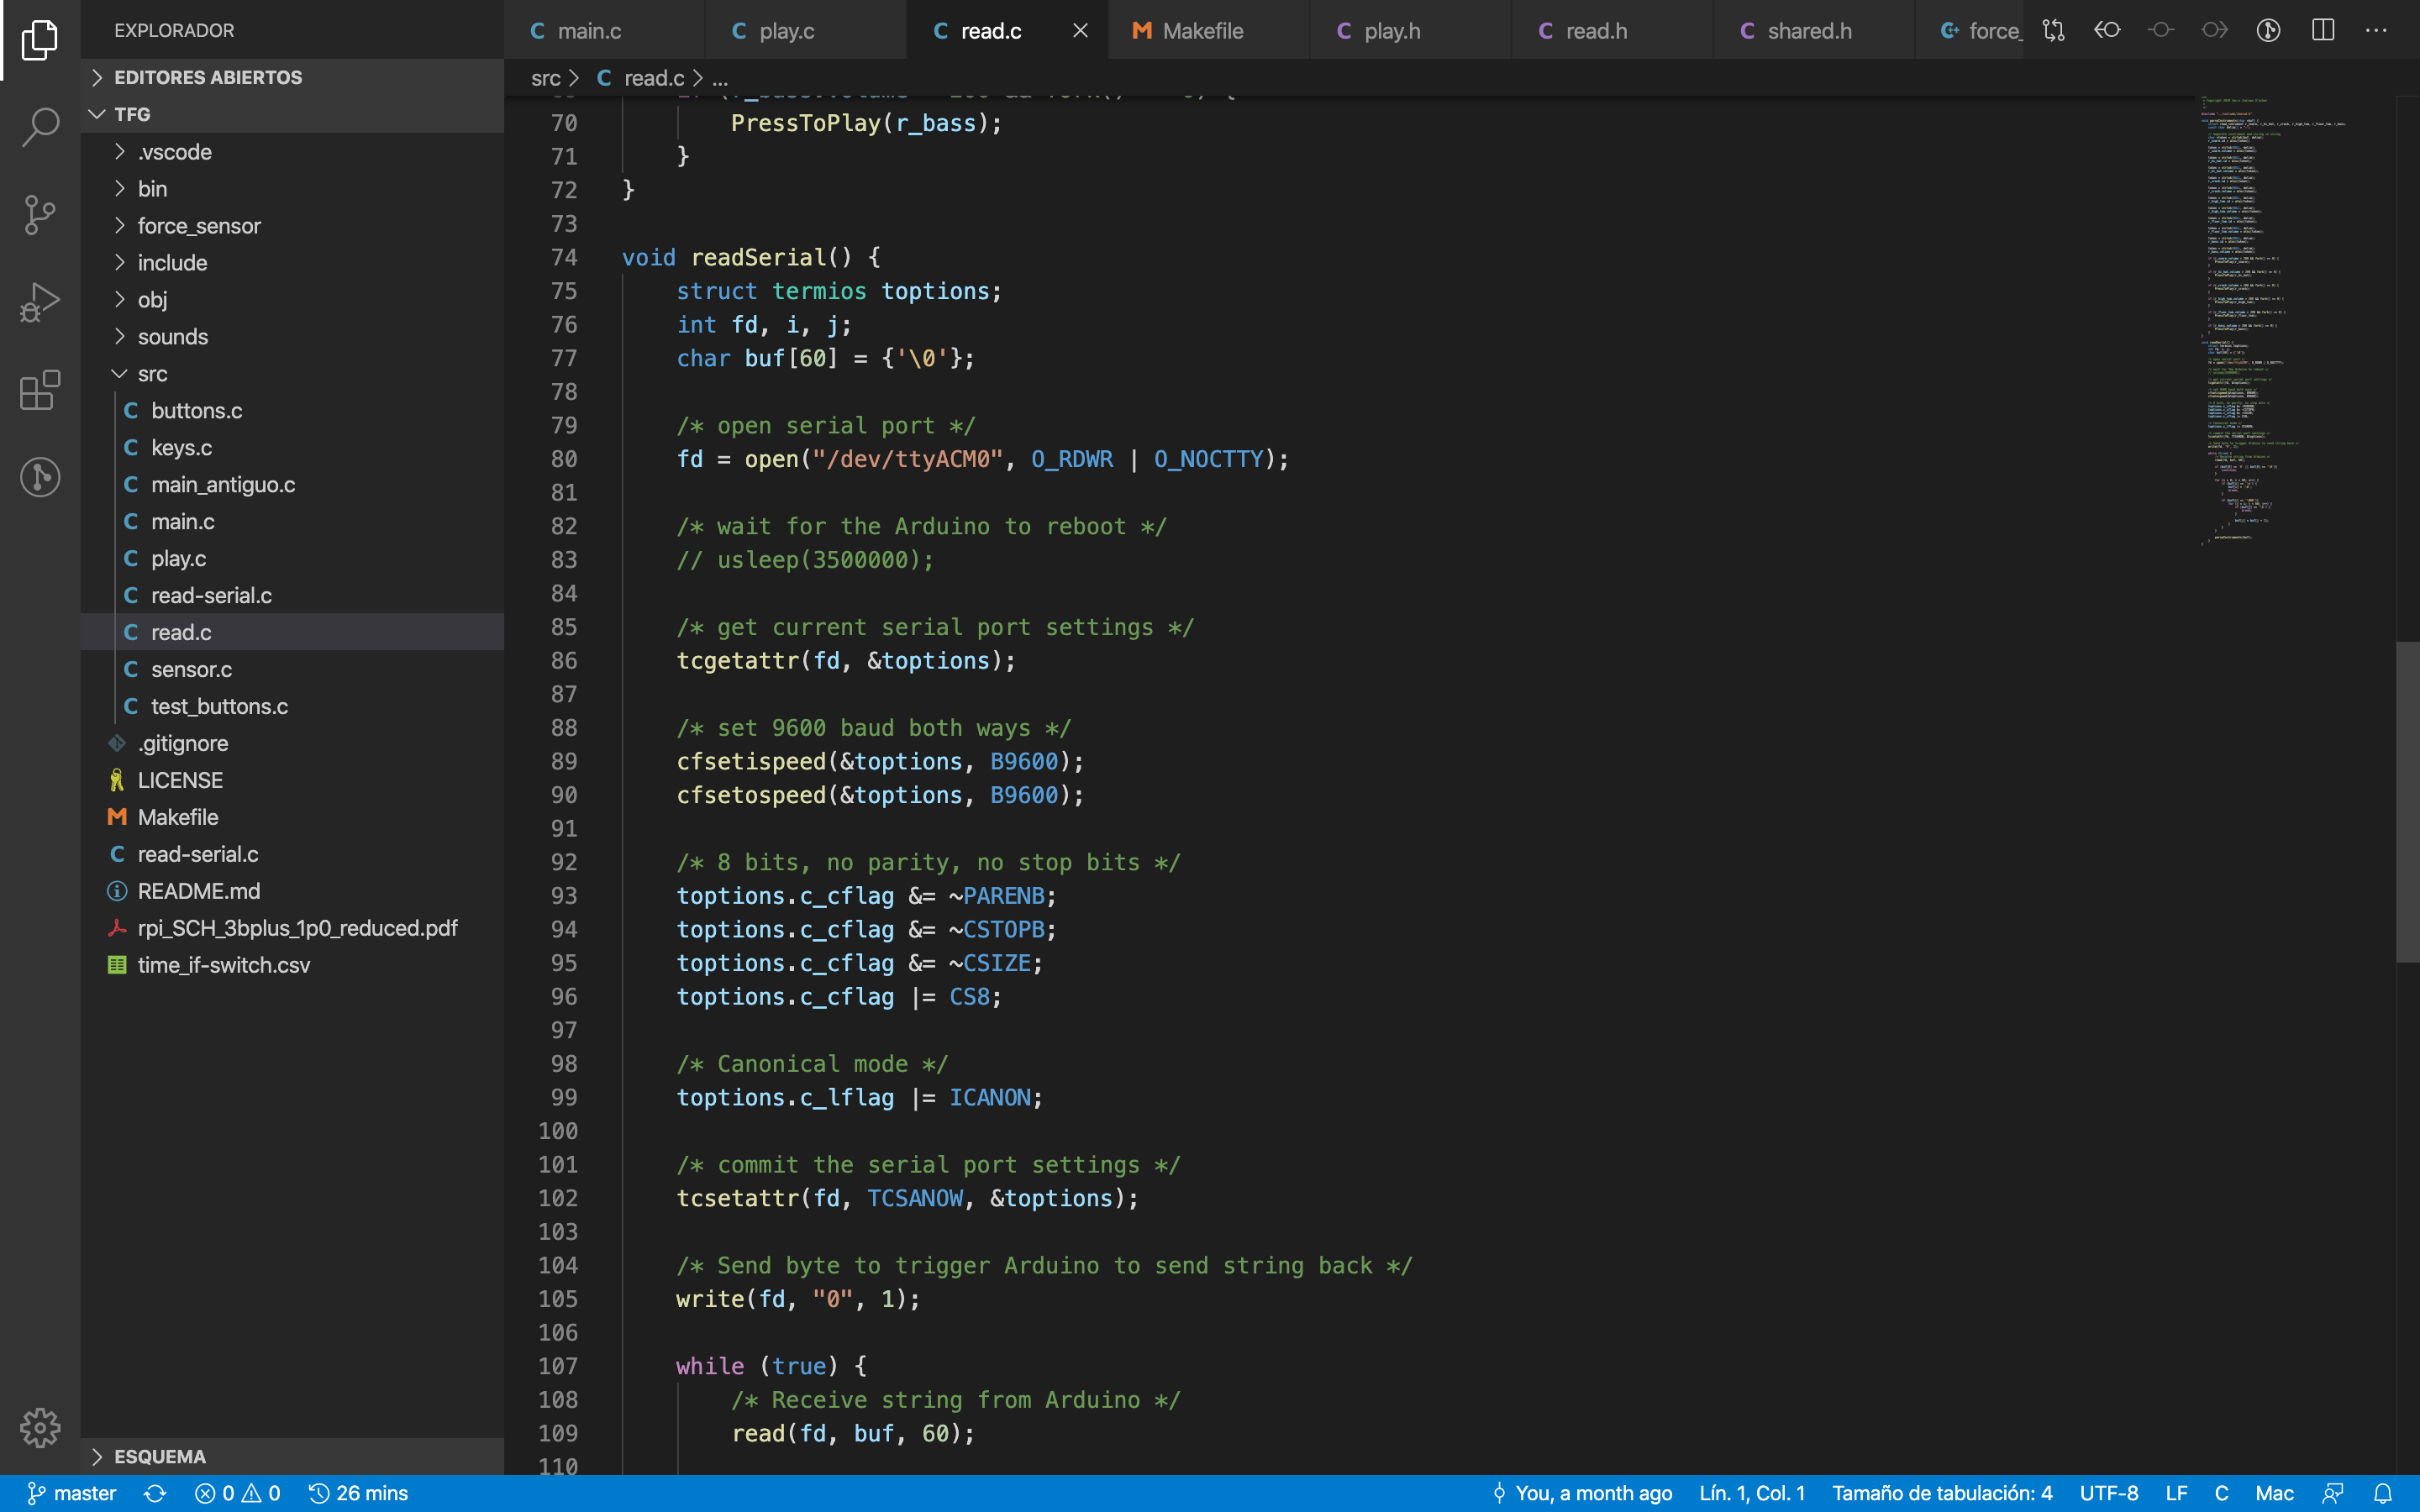
\includegraphics[width=\textwidth]{vs_code}
                \caption{Captura de pantalla de Visual Studio Code \label{fig:VisualStudioCode}}
            \end{figure}

            \newpage

        % subsection Visual Studio Code (end)

        \subsection{Github} % (fold)
        \label{sub:Github}

            Github es un servicio de alojamiento de código abierto y control de versiones mediante Git.

            En este proyecto se ha utilizado principalmente para llevar ese control de versiones del código y para
            organizar los diferentes pasos a dar y los errores encontrados durante el desarrollo mediante su capacidad
            de crear \textit{issue}. Aparte, Github permite el acceso al código por parte de cualquier persona y ofrece
            la posibilidad de contribuir al proyecto a todo el que quiera.

            \begin{figure}[ht]
                \centering
                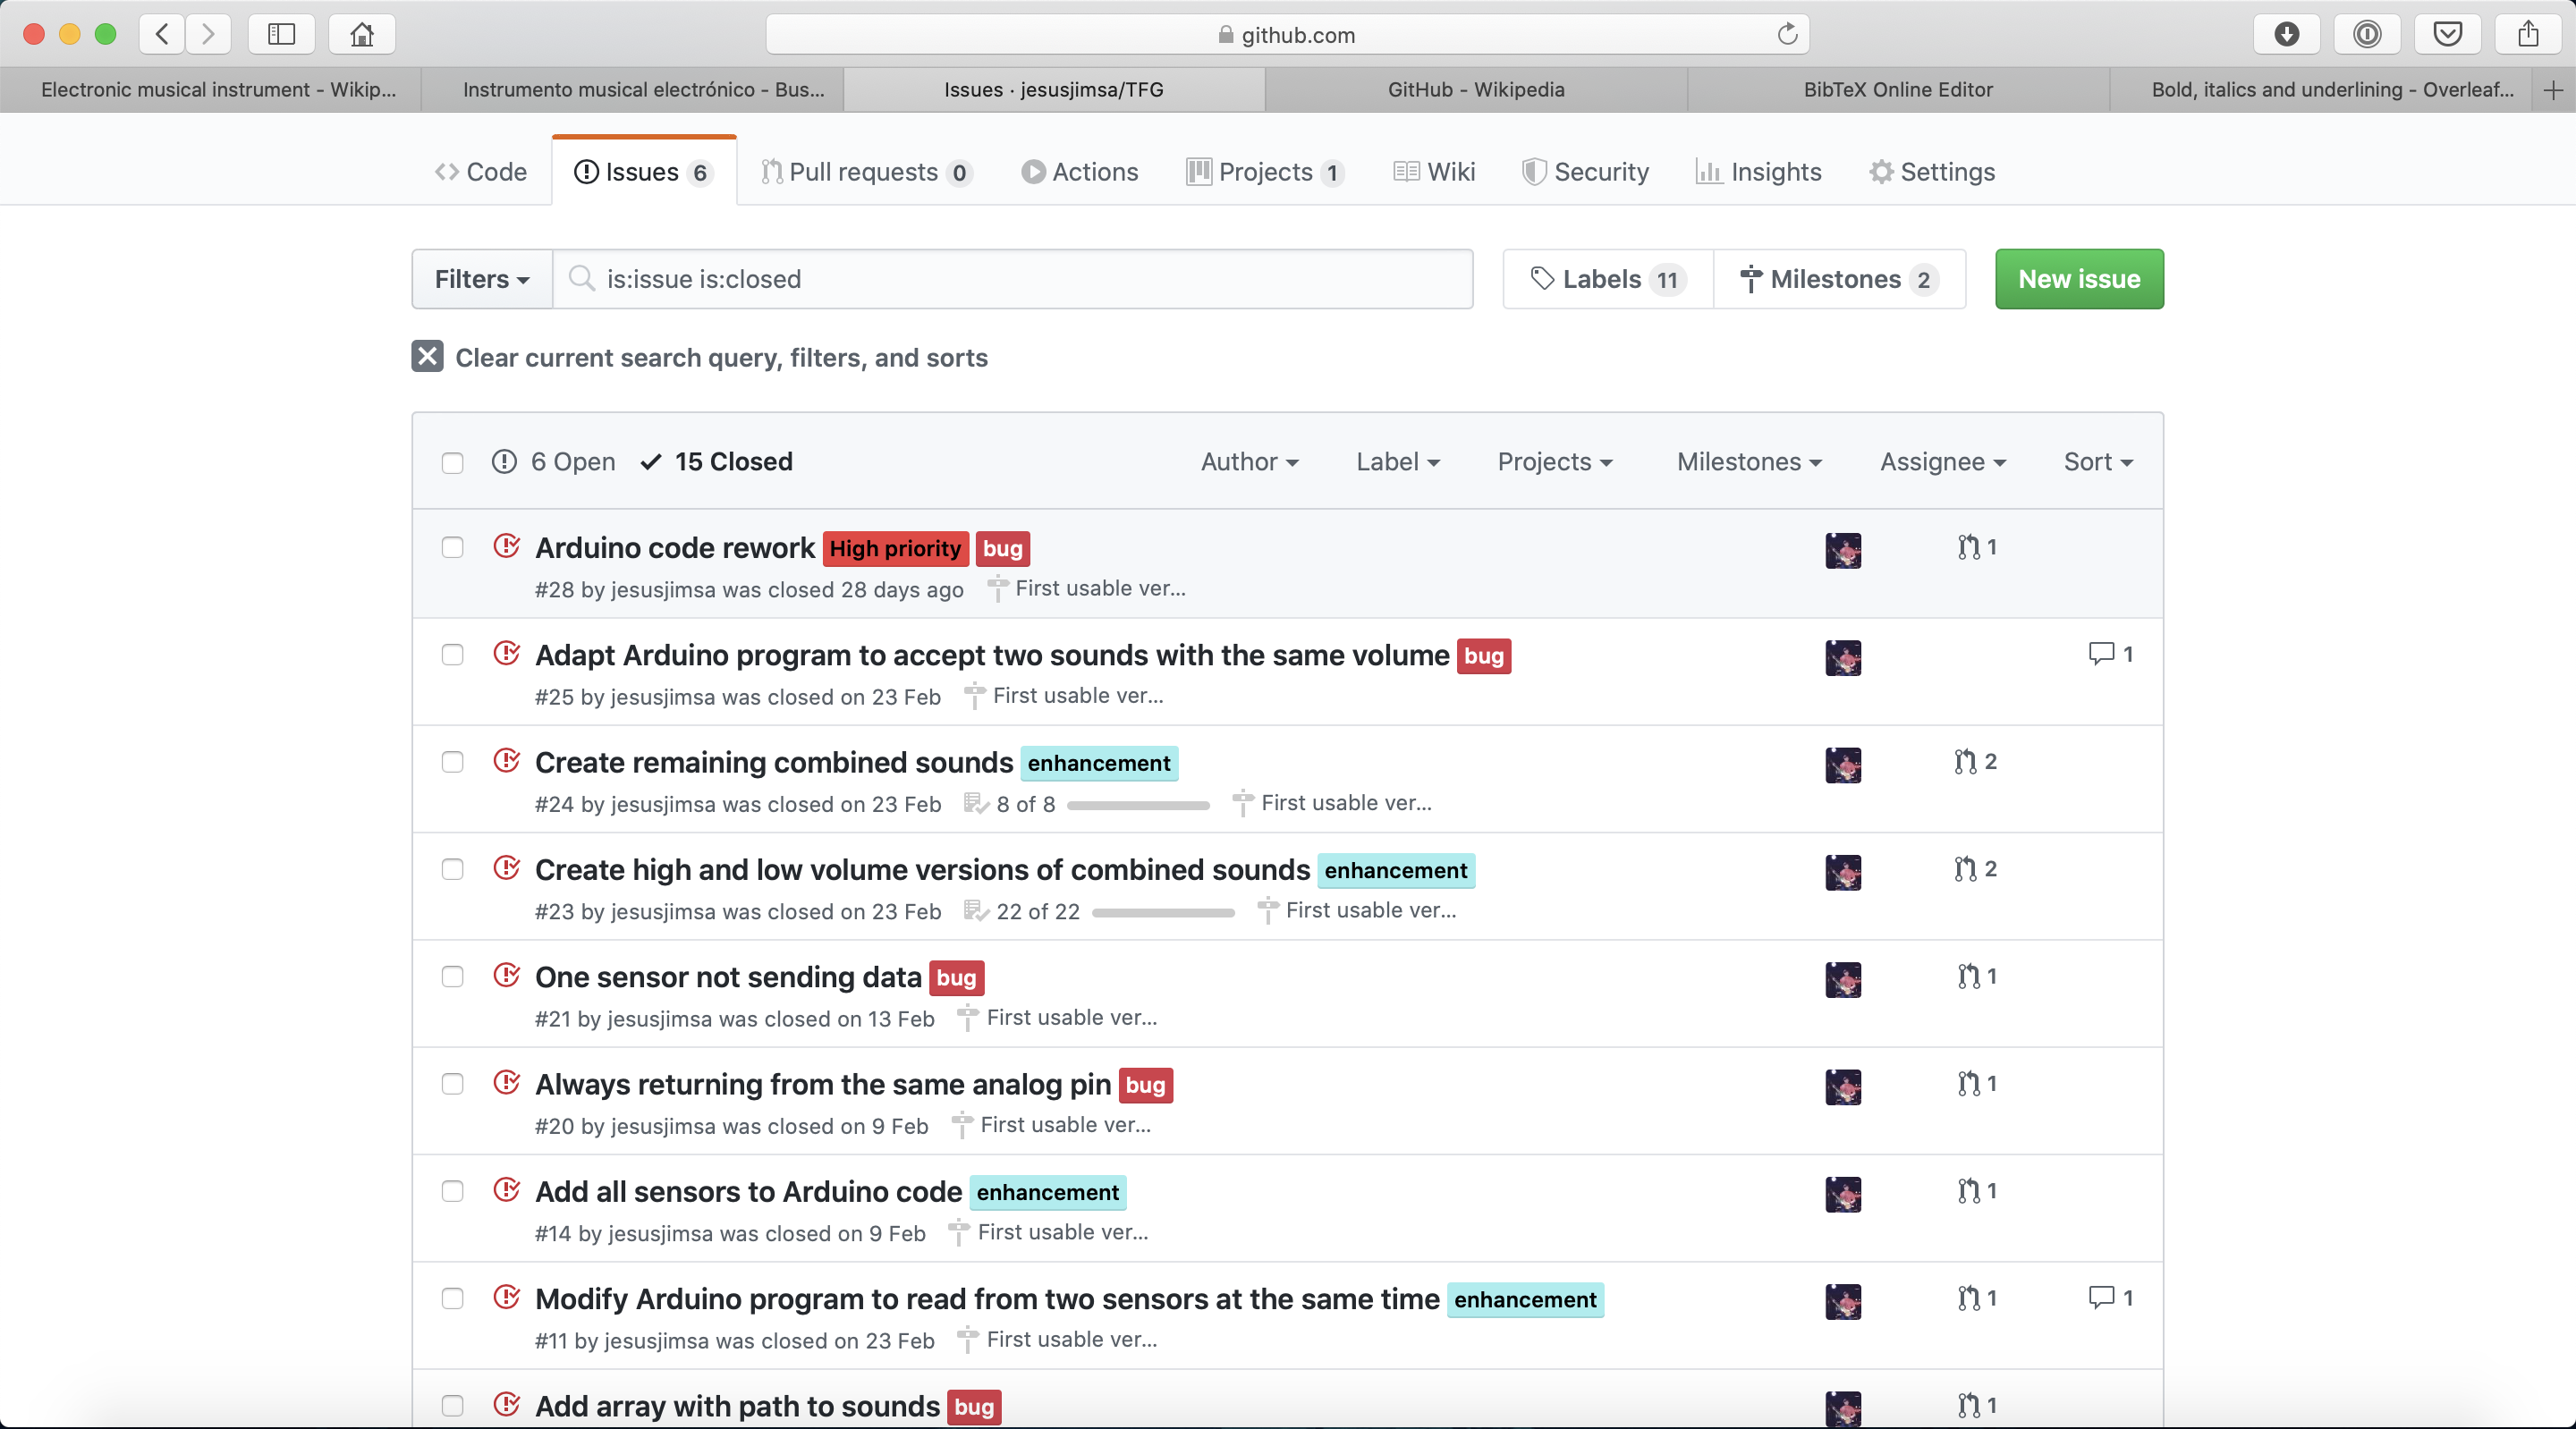
\includegraphics[width=\textwidth]{github_issues}
                \caption{Captura de pantalla de las issues de Github del proyecto \label{fig:GithubIssues}}
            \end{figure}

            \newpage

        % subsection Github (end)

        \subsection{Clockify} % (fold)
        \label{sub:Clockify}

            Clockify es una aplicación de seguimiento de tiempo. Ha sido utilizada para llevar un seguimiento de cuánto
            tiempo ha sido dedicado a la creación y desarrollo de este proyecto y su memoria.

            \begin{figure}[ht]
                \centering
                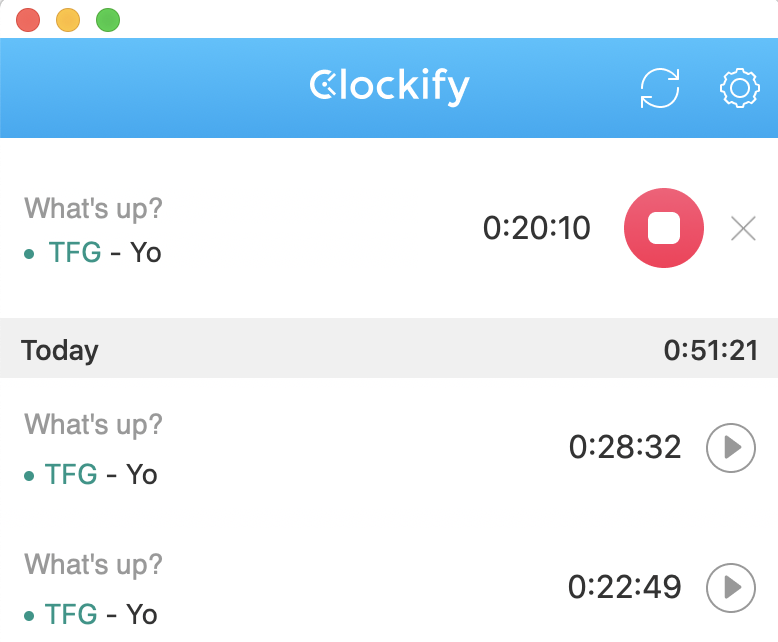
\includegraphics[width=\textwidth/2]{clockify}
                \caption{Captura de pantalla de Clockify \label{fig:ClockifyCaptura}}
            \end{figure}

        % subsection Clockify (end)

        \subsection{Overleaf} % (fold)
        \label{sub:Overleaf}

            Overleaf es un editor de LaTeX online y colaborativo. Permite crear documentos en LaTeX y la colaboración de
            hasta dos personas en su modalidad gratuita.

            En este proyecto, ha facilitado la compartición de esta memoria entre alumno y tutor para su corrección, a
            parte de servir como editor principal de LaTeX.

            \begin{figure}[ht]
                \centering
                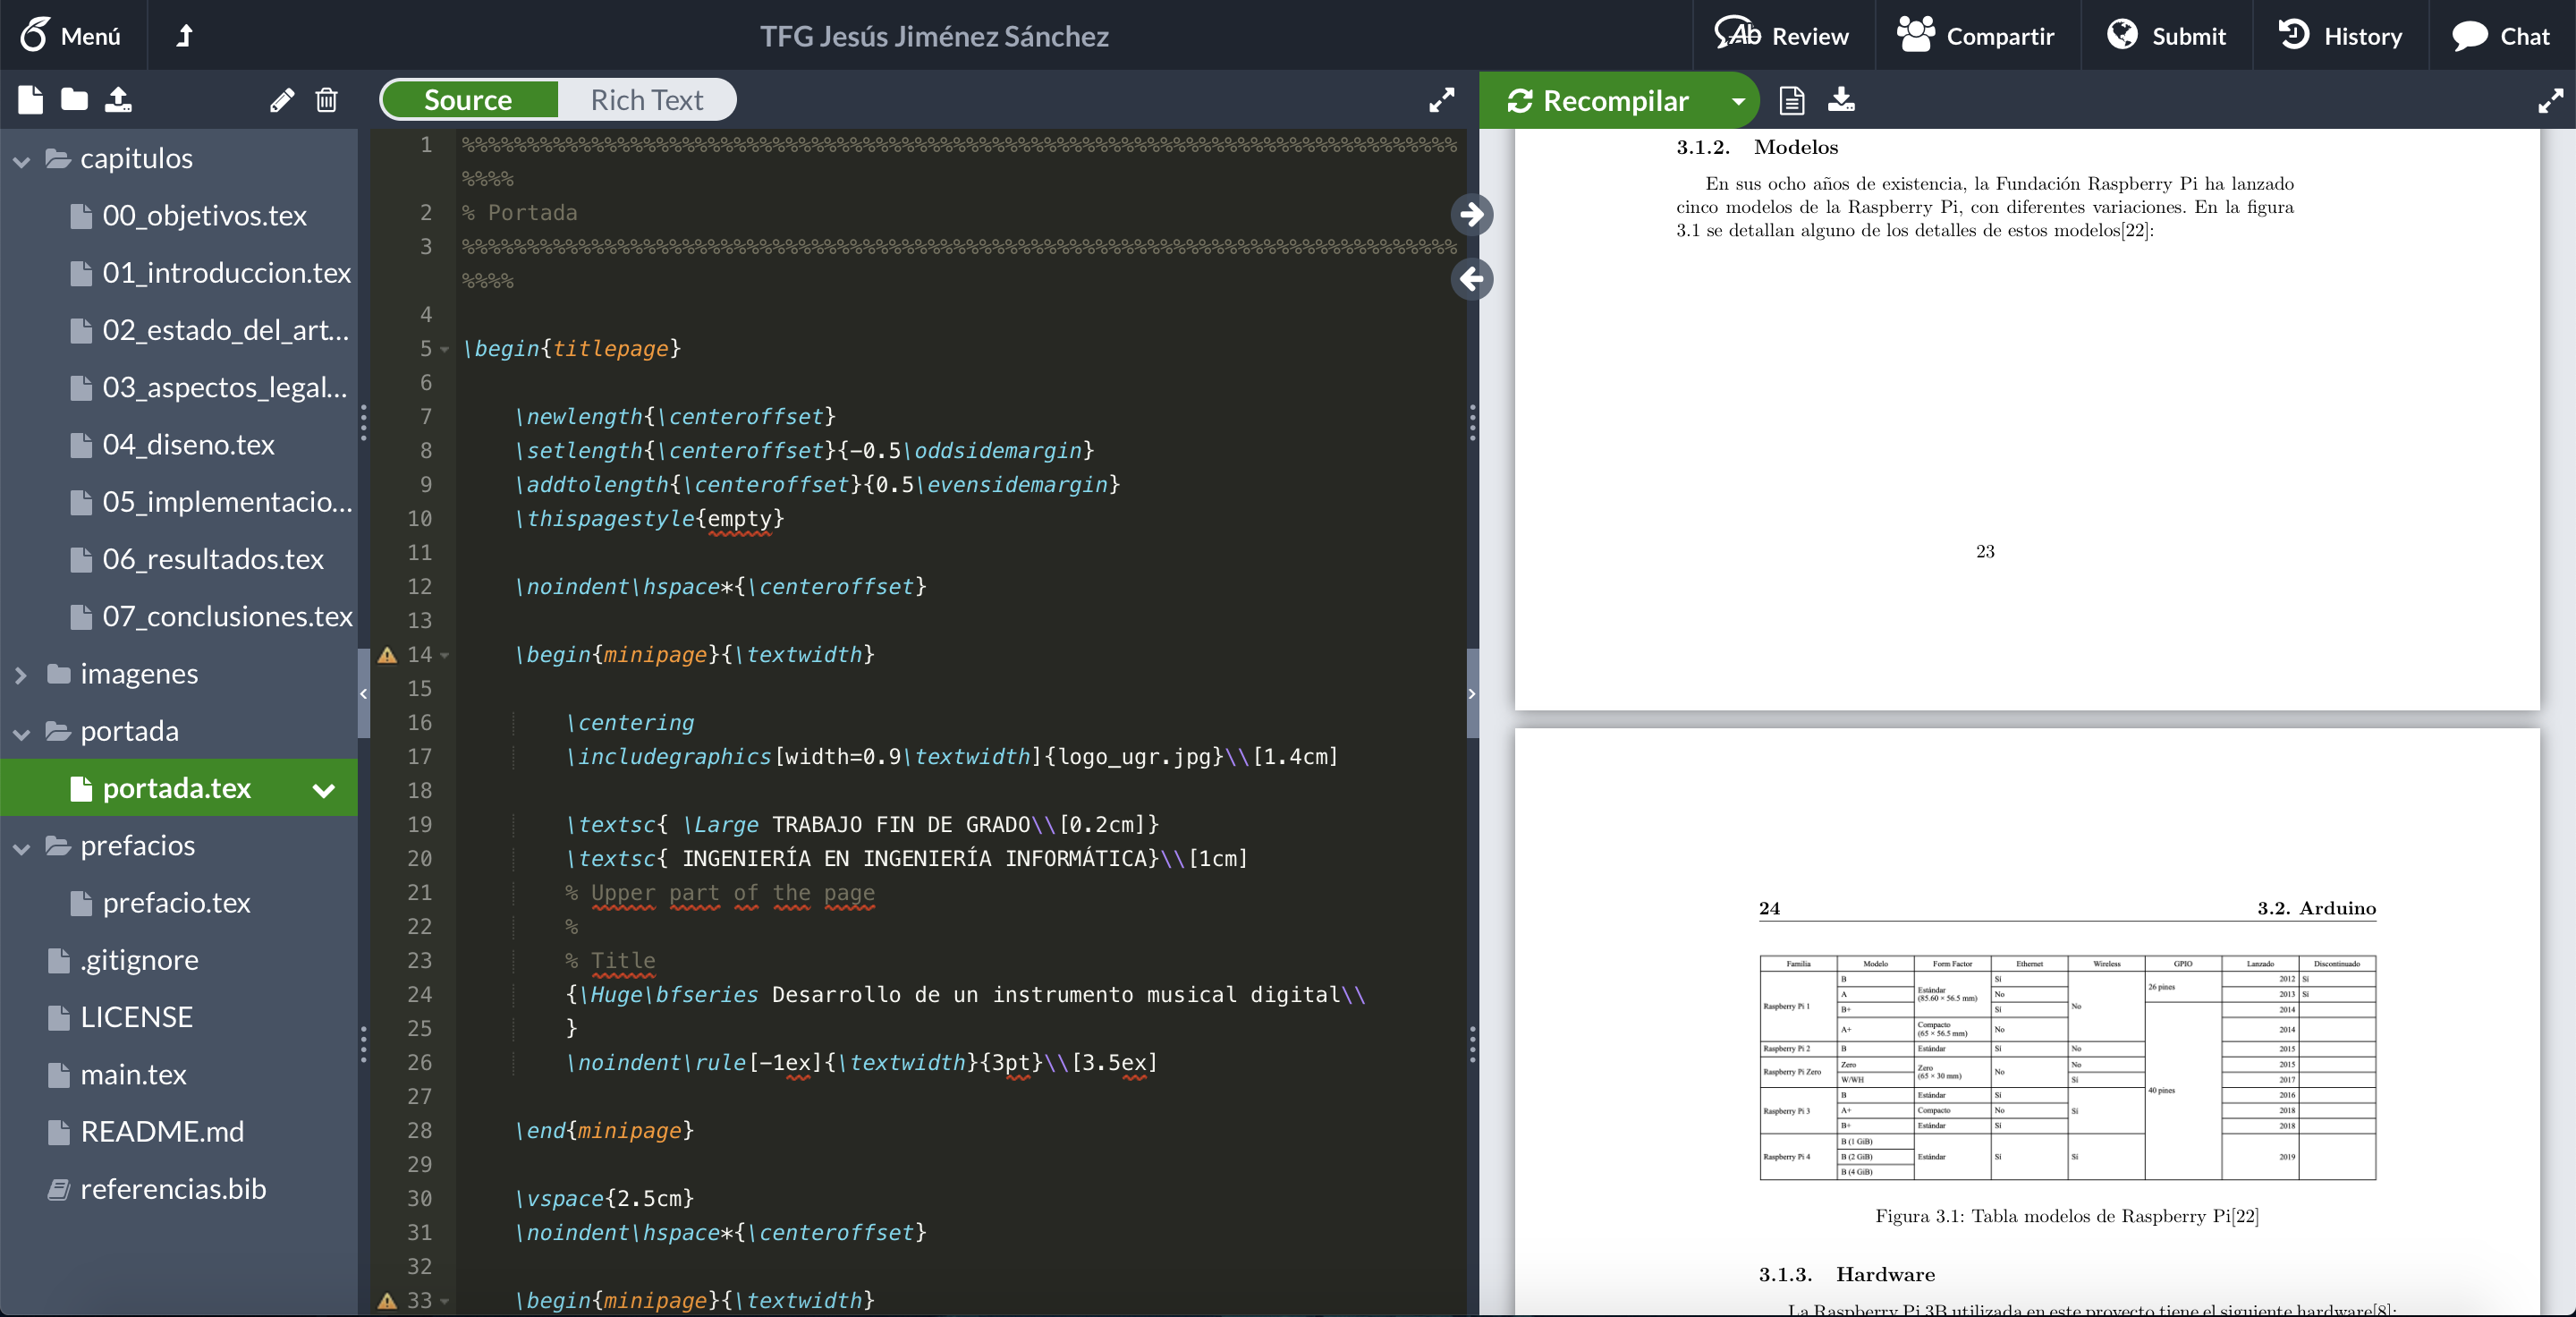
\includegraphics[width=\textwidth]{captura_overleaf}
                \caption{Captura de pantalla de Overleaf \label{fig:OverleafCaptura}}
            \end{figure}

        % subsection Overleaf (end)

    % section Tecnologías empleadas (end)

    \section{Descripción a alto nivel} % (fold)
    \label{sec:DescripcionAAltoNivel}

        La solución propuesta consta de dos partes principales. La primera parte es la recogida de información y la
        segunda, el tratamiento de la información y reproducción del sonido.

        \subsection{Recogida de información} % (fold)
        \label{sub:RecogidaDeInformacion}

            En esta primera fase se recoge la información que devuelven los sensores de fuerza en la placa Arduino. Los
            cinco sensores se conectan a la Arduino y devuelven un valor entre 0 y 1023. Este valor se junta a los
            valores leídos por todos los sensores y se manda en un solo mensaje a la Raspberry Pi para empezar la
            segunda fase.

            \newpage

            \begin{figure}[ht]
                \centering
                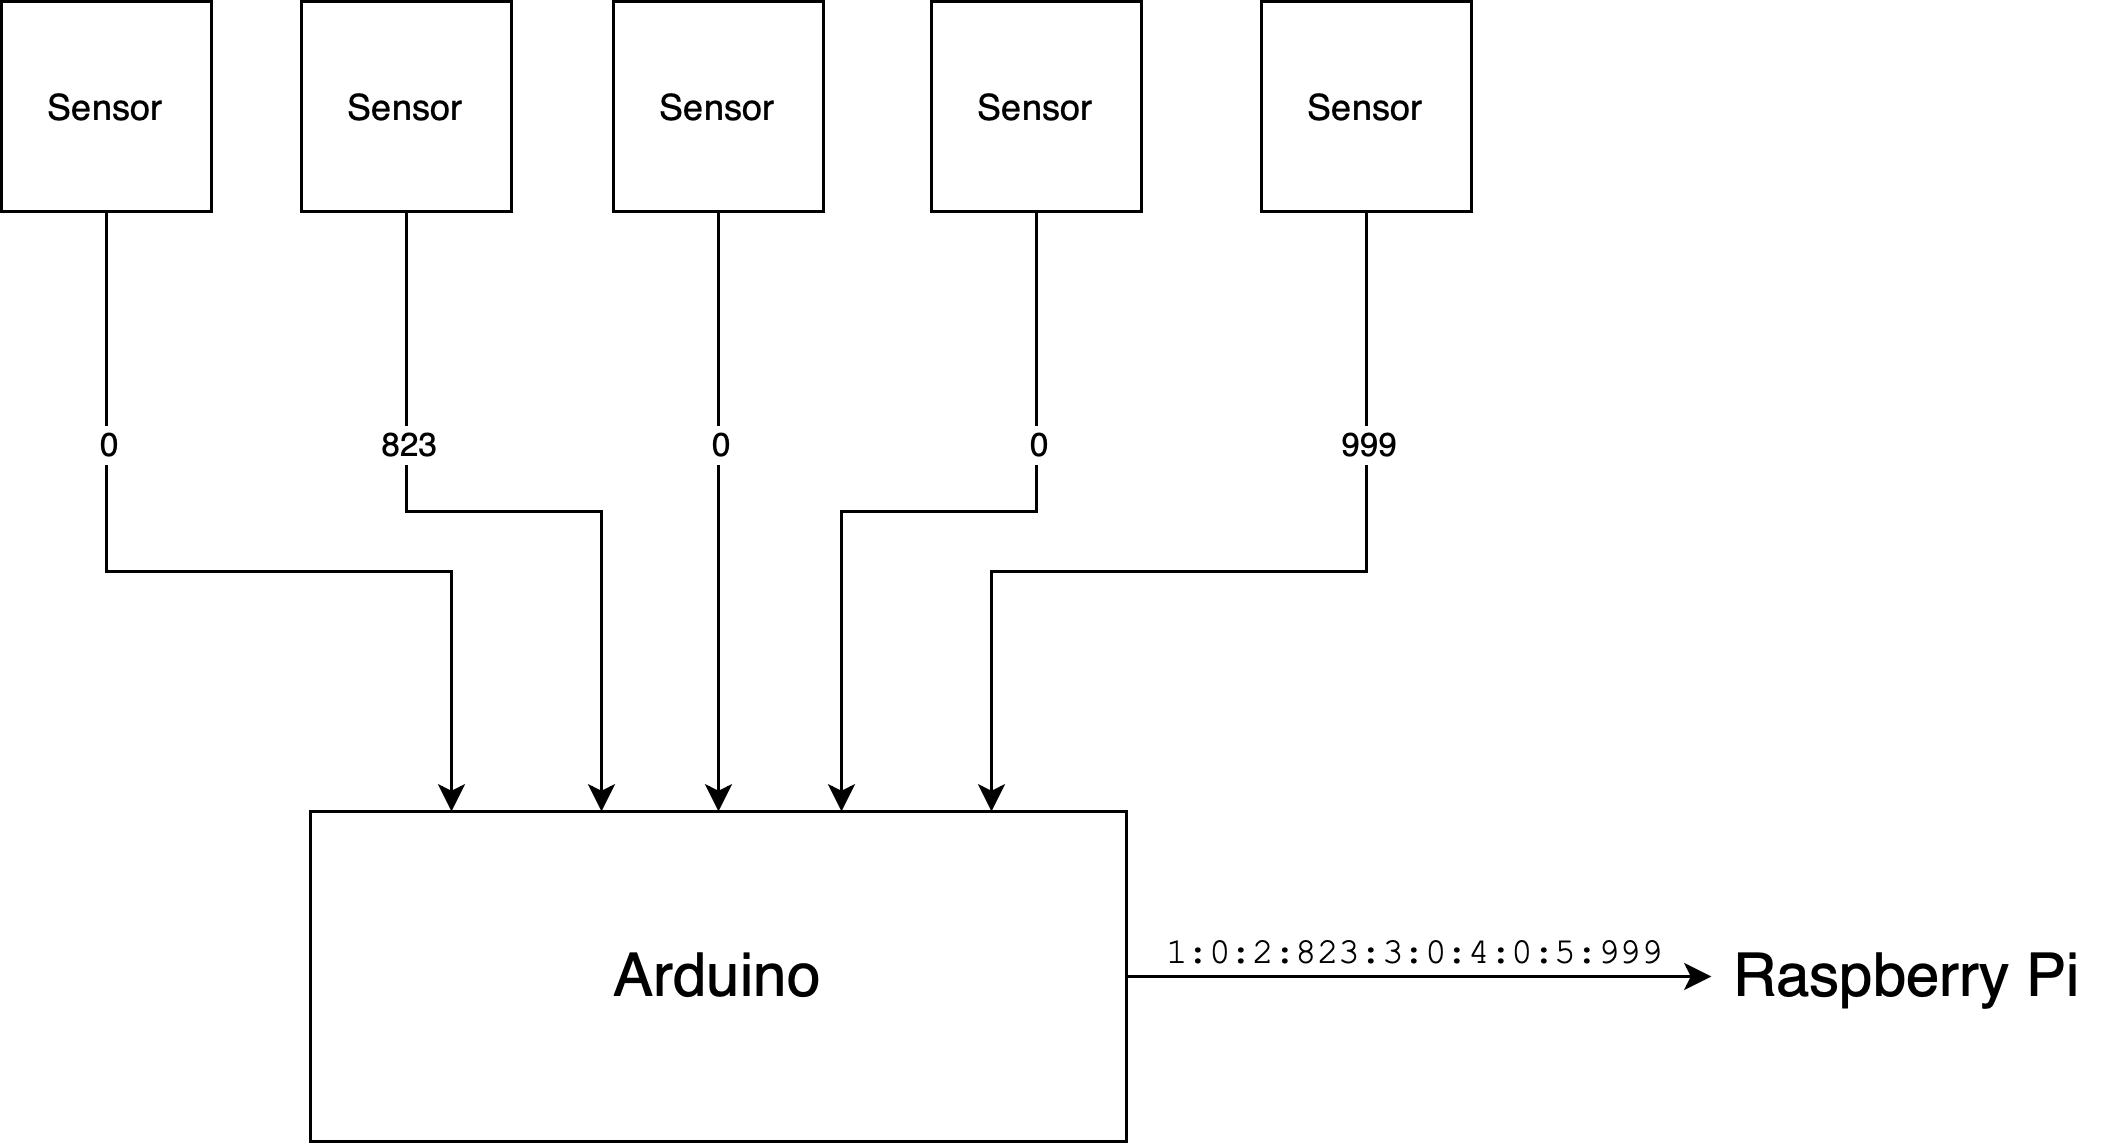
\includegraphics[width=10cm]{flow_arduino}
                \caption{Diagrama de la recogida de información \label{fig:DiagramaRecogida}}
            \end{figure}

        % subsection Recogida de información (end)

        \subsection{Tratamiento de la información y reproducción del sonido} % (fold)
        \label{sub:TratamientoDeLaInformacionYReproduccionDelSonido}

            En esta segunda parte, se recibe la información recogida por la Arduino y se reproducen los sonidos de
            batería correspondientes. La Arduino envía un mensaje por el log del monitor serie y la Raspberry Pi analiza
            este mensaje. Una vez separado el mensaje en pares de intrumento y volumen, se reproducen los sonidos
            correspondientes.

            \begin{figure}[ht]
                \centering
                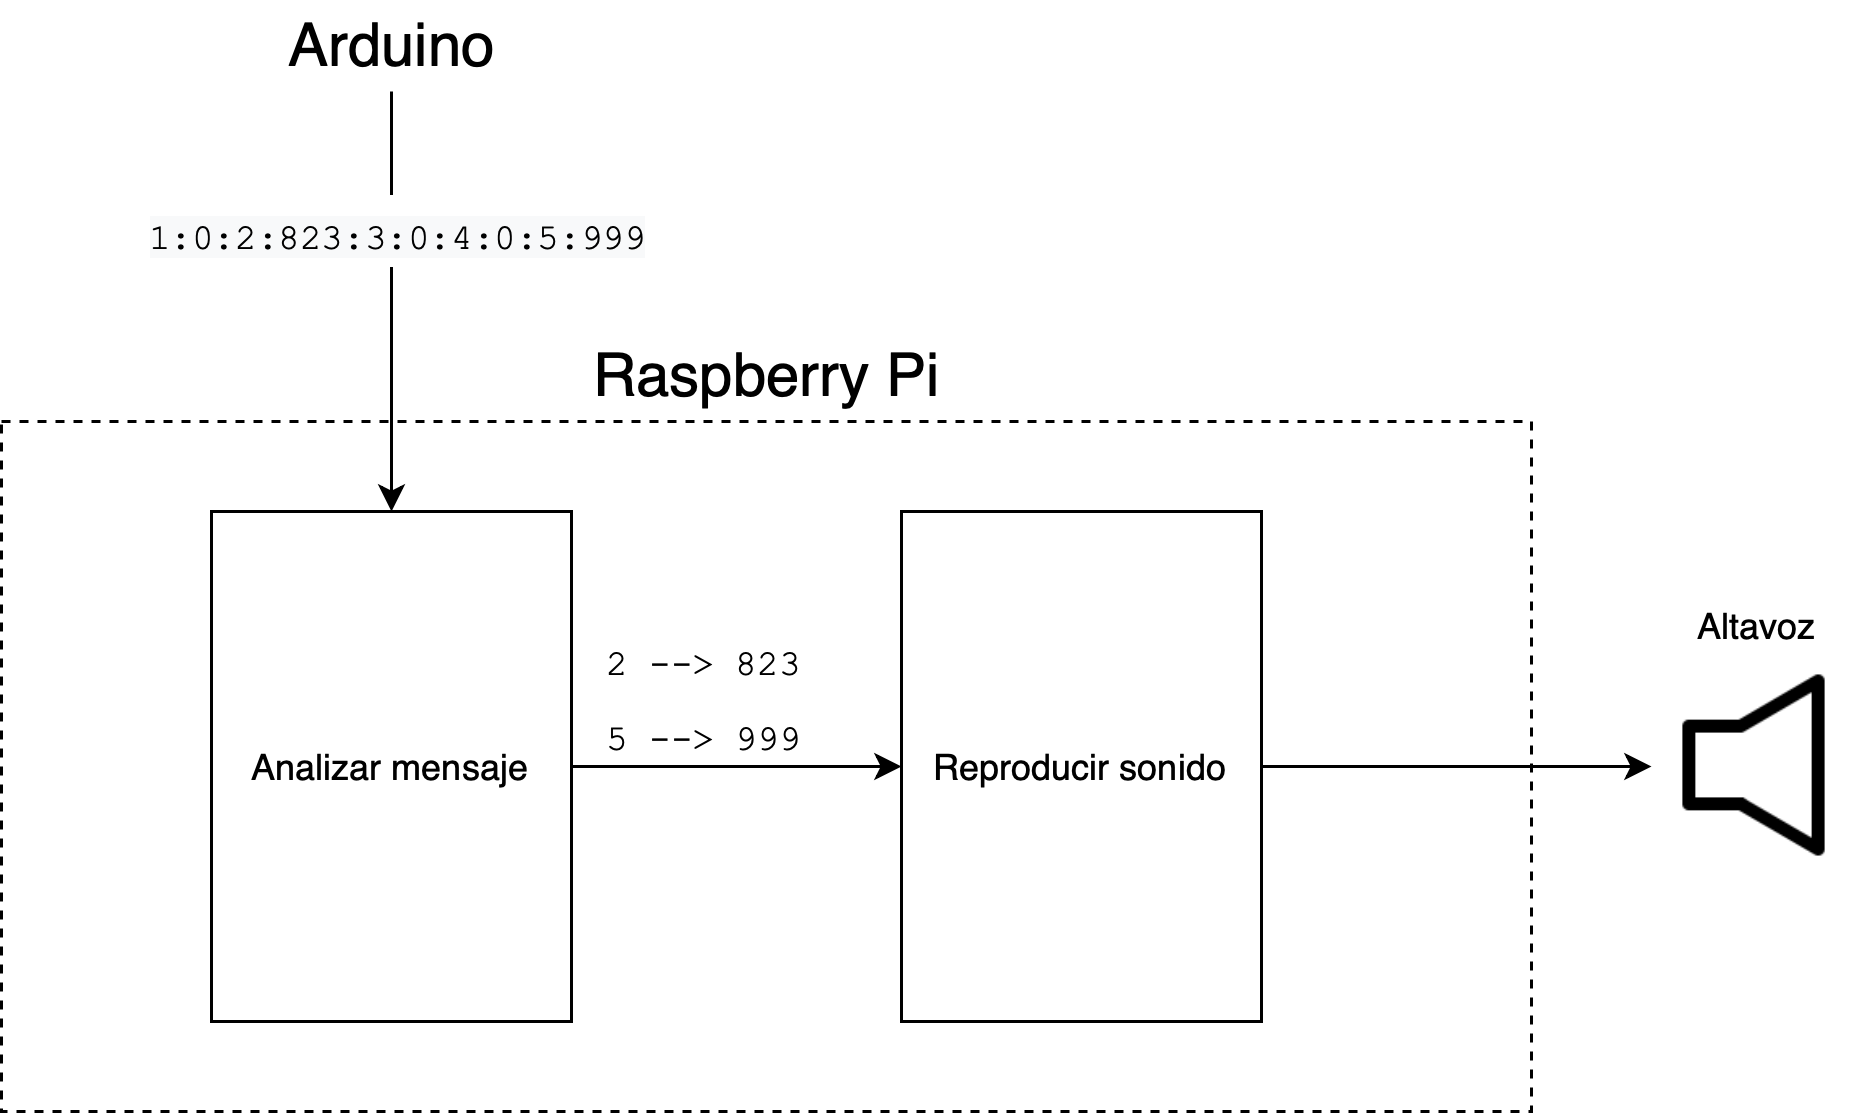
\includegraphics[width=10cm]{flow_raspberry_pi}
                \caption{Diagrama del tratamiento de la información y la reproducción del
                sonido \label{fig:DiagramaTratamiento}}
            \end{figure}

        % subsection Tratamiento de la información y reproducción del sonido (end)

    % section Descripción a alto nivel (end)

    \section{Decisiones tomadas} % (fold)
    \label{sec:DecisionesTomadas}

        La primera decisión fue entre hacer detección binaria de la entrada, es decir, si el parche ha sido golpeado o
        no, y hacer que estas entradas sean concurrentes (al golpear dos parches, el sonido de ambos suena al mismo
        tiempo), o hacer detección de distintos sonidos en un mismo parche, dependiendo de cómo se golpee el parche (en
        el centro, en el lateral, con más o menos fuerza…) el sonido emitido es diferente.

        Se decide empezar con la primera alternativa y dejar la segunda para más adelante, en caso de tener tiempo.

        Finalmente, por temas de coste, se decide no realizar la detección de distintos en un mismo parche, ya que cada
        sensor de fuerza cuesta 10,19\euro{} por lo que añadir más sensores a cada parche haría que el precio final de
        desarrollar el proyecto se elevara demasiado.

        \subsection{Biblioteca de reproducción de sonido} % (fold)
        \label{sub:LibreriaDeReproduccionDeSonido}

            \subsubsection{playsound} % (fold)
            \label{ssub:Playsound}

                Al principio se comenzó buscando implementar el proyecto en Python, por ser un lenguaje sencillo y con
                gran variedad de bibliotecas. Sin embargo, tras probar playsound \cite{playsound}, la biblioteca de
                reproducción de sonidos más popular de Python, se decidió que era muy lenta, y en este proyecto, la
                velocidad a la que se reproducen los sonidos es primordial. Por esta razón, se descarta playsound.

            % subsubsection playsound (end)

            \subsubsection{mpg123} % (fold)
            \label{ssub:Mpg123}

                Mpg123 \cite{mpg123} es una biblioteca y programa en C más rápido que playsound de Python. Tiene el
                problema de hacer que haya fallos de memoria cuando se usan hebras para reproducir varios sonidos al
                mismo tiempo, pero se soluciona utilizando procesos en su lugar.

            % subsubsection mpg123 (end)

            \subsubsection{libao} % (fold)
            \label{ssub:Libao}

                Esta biblioteca se usa en conjunto con mpg123 para reproducir el sonido de la batería.
                mpg123 es la encargada de descodificar el archivo mp3 que contiene el sonido, mientras que
                libao \cite{libao} utiliza la información que obtiene mpg123 y manda la señal al sistema operativo para
                reproducir el audio.

            % subsubsection libao (end)

        % subsection Biblioteca de reproducción de sonido (end)

        \subsection{Otras bibliotecas} % (fold)
        \label{sub:OtrasLibrerias}

            \subsubsection{wiringPi} % (fold)
            \label{ssub:WiringPi}

                Para realizar la conexión de sensores y botones a la Raspberry Pi se utiliza la biblioteca
                wiringPi \cite{wiringPi}, que es la estándar en este tema. Esta biblioteca se ha utilizado unicamente en
                los prototipos, ya que al principio se pretendía realizar el proyecto enteramente en la Raspberry Pi,
                pero finalmente se ha utilizado una Arduino para realizar la lectura de sensores.

            % subsubsection wiringPi (end)

        % subsection Otras bibliotecas (end)

        \subsection{if-else vs switch} % (fold)
        \label{sub:if-else_vs_switch}

            Al pulsar una tecla, el número leído se envía a una función que selecciona qué sonido hay que reproducir en
            ese momento, dependiendo de qué sonido corresponda a ese número. Este proceso de selección se puede hacer
            con una estructura de \textit{if-else} anidados o con un \textit{switch-case}.

            Para decidir cuál de las dos soluciones se implementa en la versión final se realizó un test en el que cada
            vez se ejecutan más iteraciones del programa cambiando de sonido en cada una de ellas. Se empieza con 1
            iteración y se termina con 10000000 iteraciones.

            \begin{figure}[ht]
                \centering
                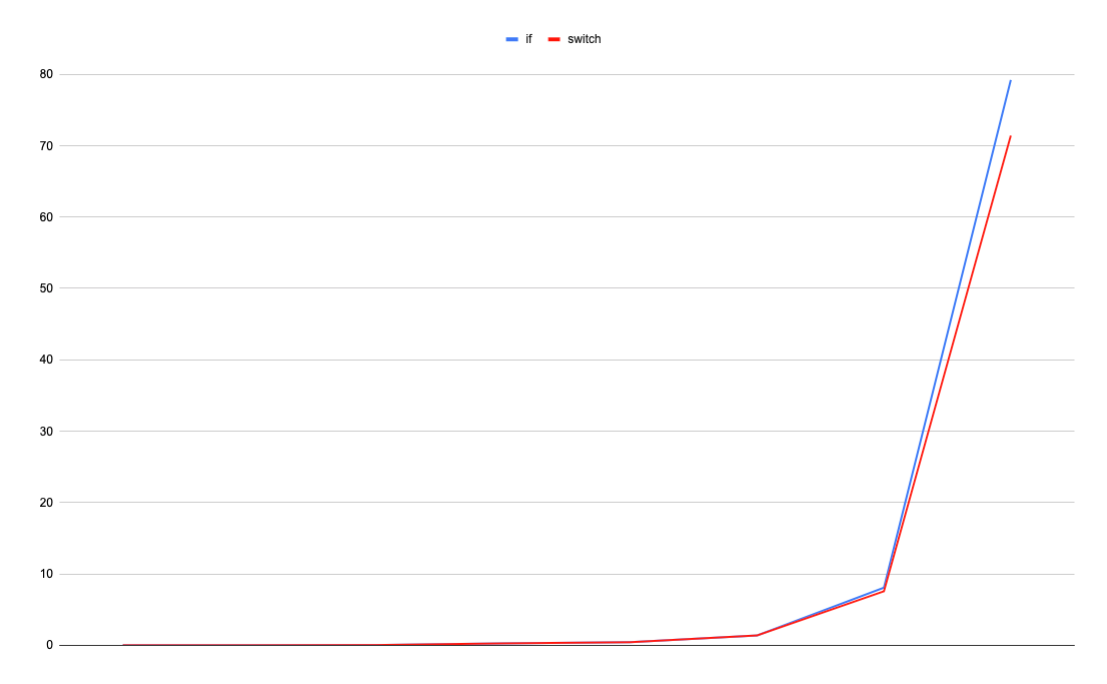
\includegraphics[width=\textwidth]{grafica_if_switch}
                \caption{Gráfica comparativa if-else vs switch \label{fig:GraficaIfVsSwitch}}
            \end{figure}

            \begin{center}
                \begin{tabular}{ |c|c|c| }
                    \hline
                        iterations & if & switch \\
                        \hline\hline
                        1 & 0.000243 & 0.000270 \\
                        \hline
                        10 & 0.002797 & 0.002485 \\
                        \hline
                        100 & 0.027775 & 0.027261 \\
                        \hline
                        1000 & 0.260075 & 0.261464 \\
                        \hline
                        10000 & 0.431544 & 0.425668 \\
                        \hline
                        100000 & 1.368561 & 1.374575 \\
                        \hline
                        1000000 & 8.070825 & 7.560718 \\
                        \hline
                        10000000 & 79.199539 & 71.409653 \\
                    \hline
                \end{tabular}
            \end{center}

            Como se puede ver en la figura \ref{fig:GraficaIfVsSwitch}, la diferencia no es apreciable hasta las
            1000000 iteraciones, pero después pasa a casi 8 segundos de diferencia en 10000000 iteraciones. Por
            esta razón se ha decidido que la función utilice la estructura \textit{switch-case}.

            Finalmente, debido a la manera en la que realizan las comprobaciones de qué botones y sensores son
            utilizados, aunque un \textit{switch-case} es más rápido, esta estructura se reserva para la versión del
            programa que reproduce los sonidos leyendo del teclado. En el programa que controla los sensores se
            utiliza una estructura \textit{if-else}.

        % subsection if-else vs switch (end)

    % section Decisiones tomadas (end)

    \section{Arduino vs Raspberry Pi} % (fold)
    \label{sec:ArduinoVsRaspberryPi}

        Para la recepción de las señales de los sensores de presión RP c18.3 y RP S40, se plantean dos opciones, se
        puede utilizar la propia Raspberry Pi en la que se ejecuta el programa que maneja los sonidos o una Arduino
        Nano. En el proyecto resultante se utiliza finalmente la Arduino debido a dos razones principales.

        La primera razón es el precio y la escalabilidad, una Raspberry Pi cuesta 39,95\euro{} mientras que una
        Arduino Nano cuesta 10\euro{}. Una Arduino Nano cuenta con menos pines de E/S, pero añadir una placa es más
        barato y sencillo que añadir una placa de Raspberry Pi.

        La segunda razón es la implementación del programa que se encarga de el sensor de presión. En Internet se
        pueden encontrar ejemplos y tutoriales refiriéndose a cómo implementar el sistema en una Arduino, pero no
        es tan fácil encontrar información para hacerlo desde una Raspberry Pi.

        Por estas razones se elige realizar la recepción de las señales del sensor de presión desde la Arduino,
        haciendo el proceso más sencillo y más barato.

        \subsection{Conexión} % (fold)
        \label{sub:Conexion}

            Para realizar la conexión de los sensores se utilizan cables de protoboard conectados de la forma
            explicada en la figura \ref{fig:EsquemaConexion}:

            \begin{figure}[ht]
                \centering
                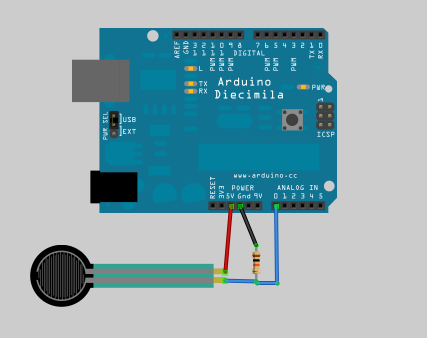
\includegraphics[width=7cm]{force_sensor_arduino}
                \caption{Esquema de conexión de sensores de presión \cite{force_sensor_arduino}
                         \label{fig:EsquemaConexion}}
            \end{figure}

        % subsection Conexión (end)

    % section Arduino vs Raspberry Pi (end)

% chapter Diseño (end)

\newpage
